\chapter{Locating RR peaks}

In this section we develop and evaluate methods for identifying QRS complexes otherwise known as RR peaks in ECG data.
The method we develop is inspired by the Pan-Tompkin Algorithm \cite{pan1985real}. The Pan-Tompkins algorithm is widely used in 
literature for ECG analysis, \cite{fariha2020analysis}, hence why we use it as inspiration in this project. 
We implement simplifications of the process whose performance we evaluate against the QRS annoations supplied.  

\section{Filtering and Pre-Processing}
ECG signals are prone to noise, and variation in the data, so its important to filter and pre-process before attempting 
to locate RR peaks. The filtering is based off literature values for ECG signals, specifically 
we expect to be locating frequencies associated within the range of 5 - 15 Hz \cite{pan1985real}. 
Figure~\ref{fig:freq_filter} illustrates an example waveform before and after filtering in different frequency ranges, employing 
a Fourier Transform before removing frequencies and inverting back. \\
\begin{figure}[H]
    \centering
    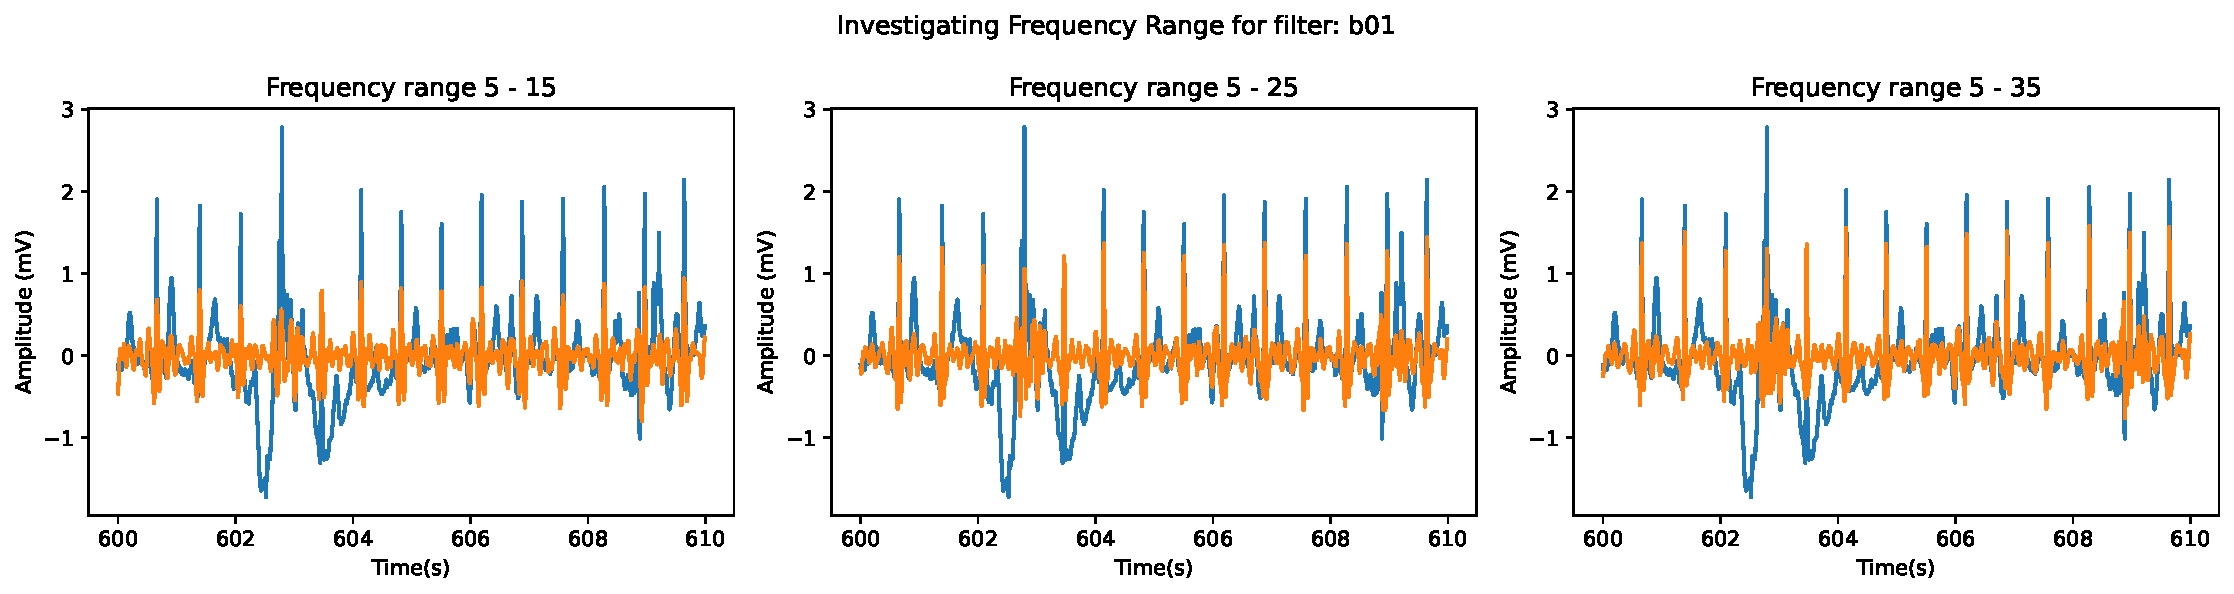
\includegraphics[width=\textwidth]{figures/Freq_filter.pdf}
    \caption{Frequency Filters applied in different ranges}
    \label{fig:freq_filter}
\end{figure}
We can see that a frequency filter cleans up the waveform to better resemble a ECG signal, whilst retaining 
the QRS complexes, Figure~\ref{fig:freq_filter} suggests that a range of 5-35 Hz best mantains 
Amplitude of the QRS complex along with an ECG signal shape, this is the frequency range this project uses.\\

Once we restrict ourselves to a filtered waveform, we implement a Pre-Processing method heavily influenced by \cite{pan1985real}. The idea 
is that RR peaks are associated with large inclines and declines in the wave form, so we want to use Derivatives, and square them to highlight and 
exhausterbate this difference, before a moving integration window converts the derivative back into a smooth signal with a large peak 
associated with the RR peaks whilst minimising the effect of the other smaller peaks. The process is specifically, 
\begin{enumerate}
        \item Differentiate the waveform.
        \item Square the differentiated waveform, to ensure all values are positive, additionally the steeper incline and decline , 
        associated with the peaks will now be amplified helping to distinguish against the smaller peaks. 
        \item A moving integration window on the Squared Differentiated waveform, produces a signal that amplifies the RR peak (nearby it), and minimises 
        the other smaller peaks. 
\end{enumerate}
Figure~\ref{fig:Pre-Process} illustrates how the waveform is transformed over this process. 
\begin{figure}[H]
    \centering
    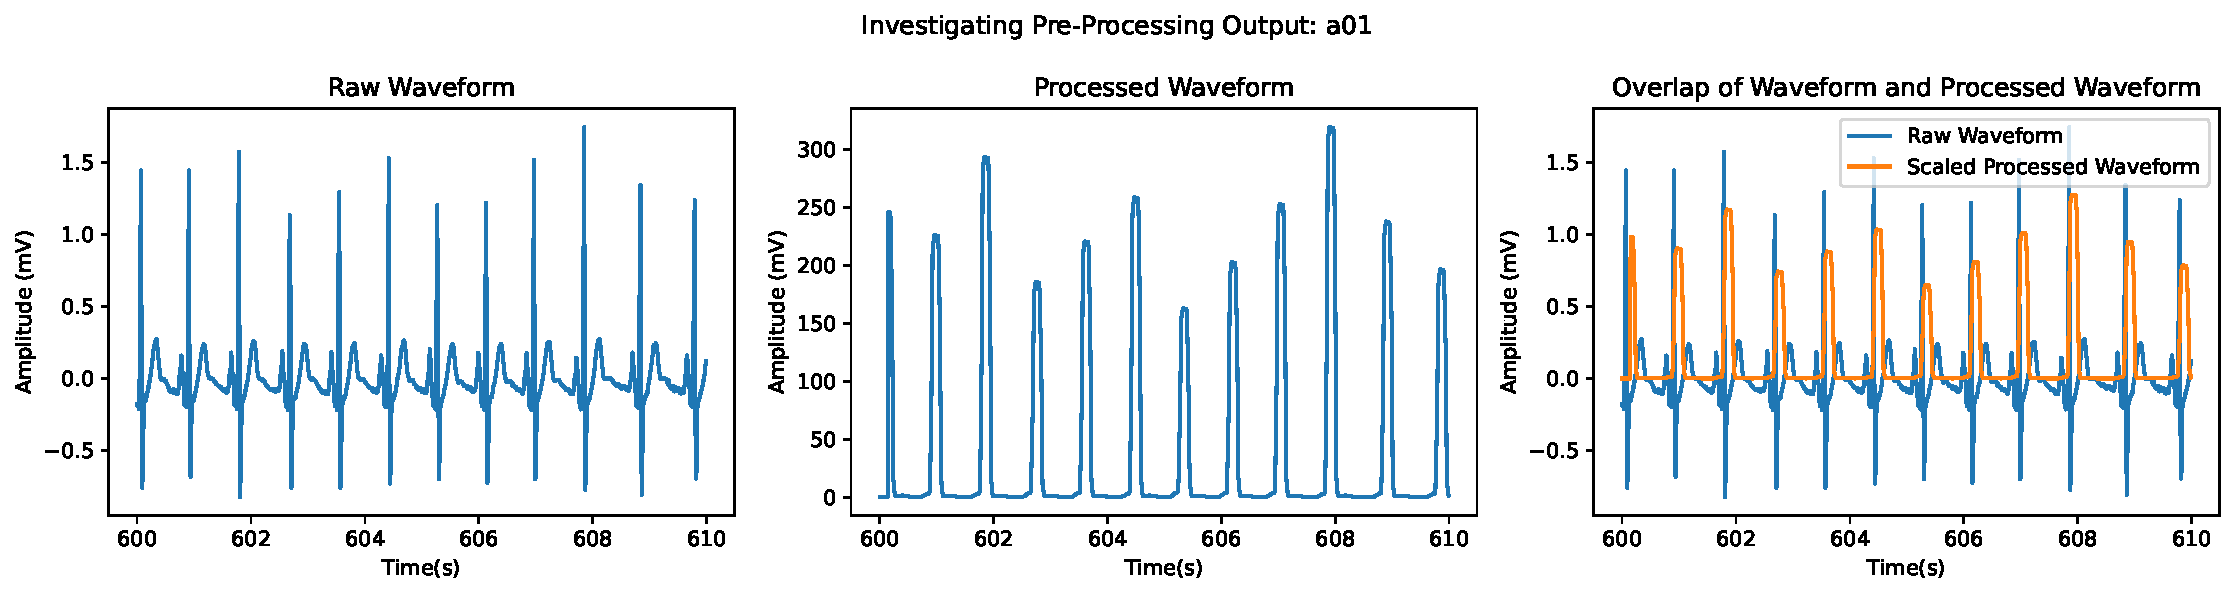
\includegraphics[width=\textwidth]{figures/Pre-Processing.pdf}
    \caption{Illustration of the Pre-Processed Waveform}
    \label{fig:Pre-Process}
\end{figure}

\section{Basic Algorithm}
We can see in Figure~\ref{fig:Pre-Process} that the processed waveform has large peaks close to (but just after) the location of the RR peaks in the Signal. The idea 
of our algorithm is to then locate the peaks on the processed waveform which are clear and can be done using an inbuilt python peaking finding function (sp.signal.find\_peaks).
We then in a small search window  around the location of these peaks, move back onto the original waveform and in this interval identify the largest value
and the time associated with it, this is what the algorithm identifies as a peak. The search window is chosen 
as 0.25 secs, this is not too large as the normal heart rate is from 60-100 bpm corresponding to 
0.6 - 1sec between QRS time complexes \cite{victorchang_resting_heart_rate}. When implementing the inbuilt function, we need to prescribe a
threshold for what we expect a peak in the integrated waveform to be above. As we have seen that amplitudes can vary significantly, the
idea of our algorithms is to then start with a high threshold value, we choose 1000 as the dataset with the largest amplitudes we identified (a13)
was roughly 700 (note the scaling is 1/200), so 1000 was chosen as a buffer. Starting from the high threshold we see how many peaks are identified, 
if not enough peaks are identified with respect to some ratio of the time interval we gradually decrease the threshold until the
number of peaks identified is above the minimum number we expect to identify. This is the basic idea of the algorithms developed in this section, Figure~\ref{fig:alg_summary} 
provides a visual summary of the Pre-Processing and search window idea. 
\begin{figure}[H]
    \centering
    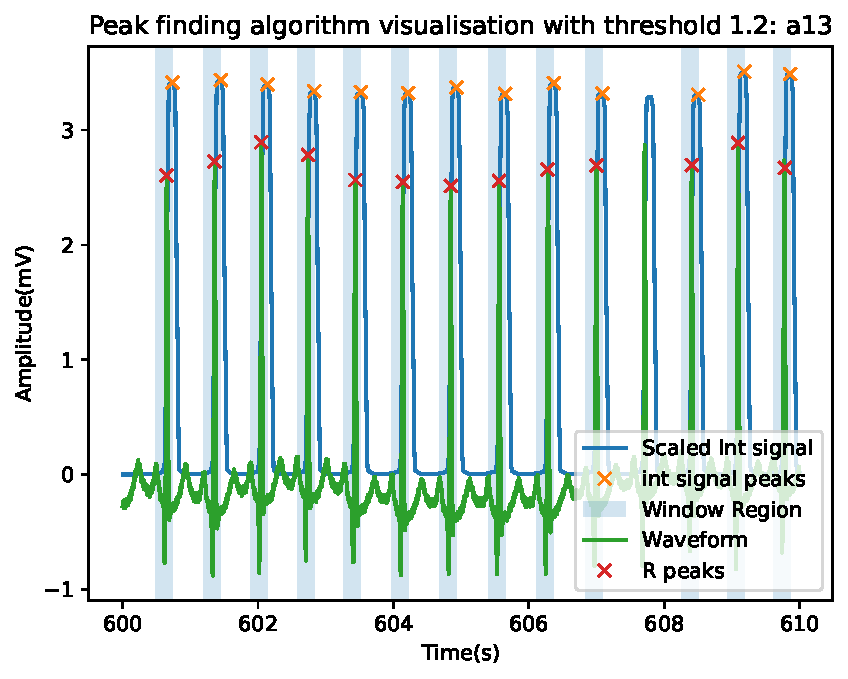
\includegraphics[width=0.5\textwidth]{figures/Algo_summary.pdf}
    \caption{Plot illustrating the basic idea of the peak finding algorithms developed in this paper}
    \label{fig:alg_summary}
\end{figure}

The pseudocode below summarises the basis idea of the base algorithm.

\begin{center}
\begin{algorithm}
\caption{Basic Algorithm form}
\begin{algorithmic}

    \State $\text{filter\_signal} \gets \operatorname{Filter}(\text{signal})$
    \State $\text{processed\_signal} \gets \operatorname{Preprocessing}(\text{filter\_signal})$
    \State $\text{threshold} \gets 1000$
    \State $\text{length\_peaks} \gets 0$

    \While{$\text{length\_peaks} < (\text{end\_time}-\text{start\_time})\text{time\_interval\_threshold}$}
        \State $\text{peaks} \gets \operatorname{find_peaks}(\text{processed\_signal}, \text{threshold})$
        \State $\text{length\_peaks} \gets \text{length}(\text{peaks})$
        \State threshold $=$ threshold $- 10$
    \EndWhile
    \For{$i = 1,\ldots,\operatorname{length}(\text{peaks})$}
    \State $\text{region} \gets \text{filter\_signal}[\text{search\_range}(i)]$
    \State peaks\_indices$[i]$ $\gets \operatorname{argmax}(\text{region})$
    \EndFor

\end{algorithmic}
\end{algorithm}
\end{center}


\section{Algorithm Evaluation}
In Figure~\ref{fig:alg_summary} we can see that with a threshold of 1.2 peaks per second that peak has been missed. To test 
which threshold is most effective, we test the number of RR peaks each algorithm identifies against the number of QRS annotations, this 
is summarised by Table~\ref{tab:threshold-results}.

\begin{table}[H]
    \centering
    \caption{Proportion of peaks detected for different threshold values between 0.8 and 1.4 in the first hour of data.}
    \label{tab:threshold-results}

    \csvautobooktabular{results_threshold_percentage.csv}

\end{table}

We can see that different time interval ratios are better than others, namely between 0.90 and 1.0, investigating between 0.90 to 1.0, we have:
\begin{table}[H]
    \centering
    \caption{Proportion of peaks detected for different threshold values between 0.9 and 1.0 in the first hour of data.}
    \label{tab:threshold-results_0.90}

    \csvautobooktabular{results_threshold_percentage_0.90_1.0.csv}

\end{table}

So the optimal number of RR peaks per second threshold value seems to be 0.90, which on average correctly identifies 88\% of peaks.


\section{Algorithm Extensions}
The problem with a fixed time interval ratio is the variability in the time between QRS complexes across
datasets. The following extensions of the algorithm described above attempt to get around this problem 
in different ways. \\

One way we could is by noticing that a large jump often occurs from values that are close to the estimated correct
number of peaks to a number far higher, intuitively this is because we are now factoring in other peaks (T, P for example).
The first extension algorithm detects this jump, and then chooses the peaks identified from the 
time interval threshold before that jump. When detecting this jump we test time interval thresholds between 
0.5 to 1.6 as the results indicate these capture all jumps we expect. Table~\ref{tab:jump-results} summarises the performance of this 
algorithm. 
\begin{table}[H]
    \centering
    \caption{Proportion of peaks detected for the jump based algorithm}
    \label{tab:jump-results}
    \csvautobooktabular{results_threshold_jump.csv}
\end{table}
Its clear from this table that this algorithm performs far better than any of 
the fixed time interval threshold based algorithms, on average it correctly identifies 101\% of 
peaks, noting that it befores well on most datasets, with notably worse performance for x04 and b02.
The sacrifice with this algorithm is that the increased complexity reduces the efficiency 
of the algorithm. Table~\ref{tab:time-results} illustrates that the run time over an hour of data increases 
up to about 15 times. 
\begin{table}[H]
    \centering
    \caption{Time Comparison (sec) for running each algorithm over an hour of data}
    \label{tab:time-results}
    \csvautobooktabular{results_time.csv}
\end{table}

\newpage

 In the basic algorithm the while loop gets replaced with the following, its clear how the time 
 complexity increases. 
\begin{algorithm}
\caption{Jump Based Modification to location of Processed Signals Peaks}
\begin{algorithmic}

    \State $\text{threshold} \gets 1000$
    \State $\text{initialise arrays to store peaks (peaks\_list) and
     number of peaks identified (peaks\_size)}$
    \For{$i = 5,\ldots,16$}
        \State $\text{time\_interval\_threshold} \gets i \times 0.1$
        \State $\text{length\_peaks} \gets 0$
        \State current\_threshold $\gets$ threshold
        \While{$\text{length\_peaks} < (\text{end\_time}-\text{start\_time})\text{time\_interval\_threshold}$}
                \State $\text{peaks} \gets \operatorname{\text{find\_peaks}}(\text{processed\_signal}, \text{threshold})$
                \State $\text{length\_peaks} \gets \text{length}(\text{peaks})$
                \State current\_threshold $=$ current\_threshold $-10$
        \EndWhile
        \State peaks\_list$[i-5]$ $\gets$ peaks
        \State peaks\_size$[i-5]$ $\gets$ length(peaks)
    \EndFor
    \State found $\gets$ False
    \For{$j = 1, \dots, \text{length(\text{peaks\_size})} - 1$}
        \If{peaks\_size$[j + 1]$ / peaks\_size$[j] \geq 2$ }
                \State peaks $=$ peaks\_list$[j]$
                \State found $\gets$ True
                \State break
        \EndIf
    \EndFor
    \If{found $=$ False}
        peaks $=$ peaks\_list$[-1]$
    \EndIf

\end{algorithmic}
\end{algorithm}


Another improvement that is only relevant to the data sets used in this project, is by 
basing the time interval threshold as a factor (something around 0.9-0.95) of the number of QRS annotations, this is clearly not 
a very viable algorithm however has it can't be used on other datasets but is worthwhile 
evaluating as is if its robust on these datasets it may be a good candidate when 
we test Respiratory Rate estimation methods. Tables~\ref{tab:QRS-results-0.9},~\ref{tab:QRS-results-0.95}
 summarise the performance of this algorithm. 
\begin{table}[H]
    \centering
    \caption{Proportion of peaks detected for the annotation based algorithm with factor 0.90}
    \label{tab:QRS-results-0.9}
    \csvautobooktabular{results_threshold_qrs_0.9.csv}
\end{table}
\begin{table}[H]
    \centering
    \caption{Proportion of peaks detected for the annotation based algorithm with factor 0.95}
    \label{tab:QRS-results-0.95}
    \csvautobooktabular{results_threshold_qrs_0.95.csv}
\end{table}

With a factor of 0.90 the average perctange of peaks detected is 93\%, and for a factor of 0.95 
it is 118\% (due to the heavy influence of b02). Here the algorithm is almost 
identical to the basic algorithm form with the modification that:
\[
\text{time interval threshold}
= \text{factor} \times
\frac{\text{number of annotations}}
{\text{end time} - \text{start time}}
\] 
Of these two possible extensions of the algorithms its clear that the jump
detection based algorithm is the best performing, with a sacrifice on efficiency -
which gets amplified in the Respiratory Rate estimation process. 



